\documentclass[11pt, a4paper, fleqn]{article}

\usepackage{CJKutf8}
\usepackage{framed}
\usepackage{graphicx}
\usepackage{caption}
\usepackage{physics}
\usepackage{url}
\usepackage[hidelinks]{hyperref}
\usepackage[style=ieee, citestyle=numeric-comp]{biblatex}
\ExecuteBibliographyOptions{
	sorting=none,
	maxnames=3,
	minnames=2,
	abbreviate=true,
	doi=false,
	}
%\AtEveryBibitem{\clearfield{title}} % Uncomment to eliminate titles in the Bibliography
\addbibresource{example.bib} % Put your biblatex file in the same directory as main.tex

%
\usepackage[hmargin=19.05truemm,vmargin=25.40truemm]{geometry}
\captionsetup[figure]{
	format=plain,
	labelformat=simple,
	labelsep=period,
	font={up, footnotesize}
	}
%
\newcommand*{\JaTitle}[1]{\begin{CJK}{UTF8}{ipxm}#1\end{CJK}}

\emergencystretch=1em

\newcommand{\figref}[1]{Figure~\ref{#1}}
\newcommand{\tabref}[1]{Table~\ref{#1}}
\renewcommand{\eqref}[1]{Equation~(\ref{#1})}

\begin{document}

	\twocolumn[
		\begin{framed}  %{screen} for rounded-corner frame
    \vspace{5pt}
    \begin{CJK}{UTF8}{ipxm}融合情報学調査輪講 % or 融合情報学成果輪講
         \hspace{\fill} yyyy月mm月dd日 % date
        \end{CJK}
    \begin{center}
        \vspace{5pt}
        {\Large 
        RINKO title in English %Title En
        } \\
        \vspace{5pt}
        {\bf \begin{CJK}{UTF8}{ipxm}
        日本語タイトル %Title ja
        \end{CJK}} \\
    \end{center}
    \vspace{5pt}
    \begin{CJK}{UTF8}{ipxm}指導教員\ \ professor name % name of your supervisor 
        \hspace{\fill} 博士1年\ \ 37-xxxxxx\ \  your name % Your grade, student id and name
    \end{CJK}
    \vspace{5pt}
\end{framed} \vspace{5pt}
		]

	
	\noindent {\large \bf Abstract\ \ }  
% put your abstract text
This is a latex format for EEIS RINKO. Modify title.tex, abstract.tex here and chapter files.
	\section{Section title}

\subsection{Subsection title}

\subsubsection{Subsubsection title}
Subsubsection with numbering.

\subsubsection*{Subsubsection title}
Subsubsection without numbering.
	\section{Examples}
Use the following examples when you use equations, figures and tables.

\section{Equation}
You can put inline equation with \$ like $E=mc^2$. If you use equation or align environment, you can display equations as following:
\begin{align}
    L_p^{|\ell|}(x) = \sum_{r=0}^{p}(-1)^r\mqty(p+|\ell|\\p-r)\cfrac{x^r}{r!}. \label{eq:laguerre}
\end{align}
You can refer exiting equation with labels defined in the equation like \eqref{eq:laguerre}.

Physics package is useful for complex equations. See \url{http://mirrors.ibiblio.org/CTAN/macros/latex/contrib/physics/physics.pdf} for more info.

\subsection{Figure}
You can use \textbackslash includegrahics to display figures, usually in figure environment. Example is shown in \figref{fig:einstein}.
\begin{figure}[htbp] % htbp: position controller
    \centering
    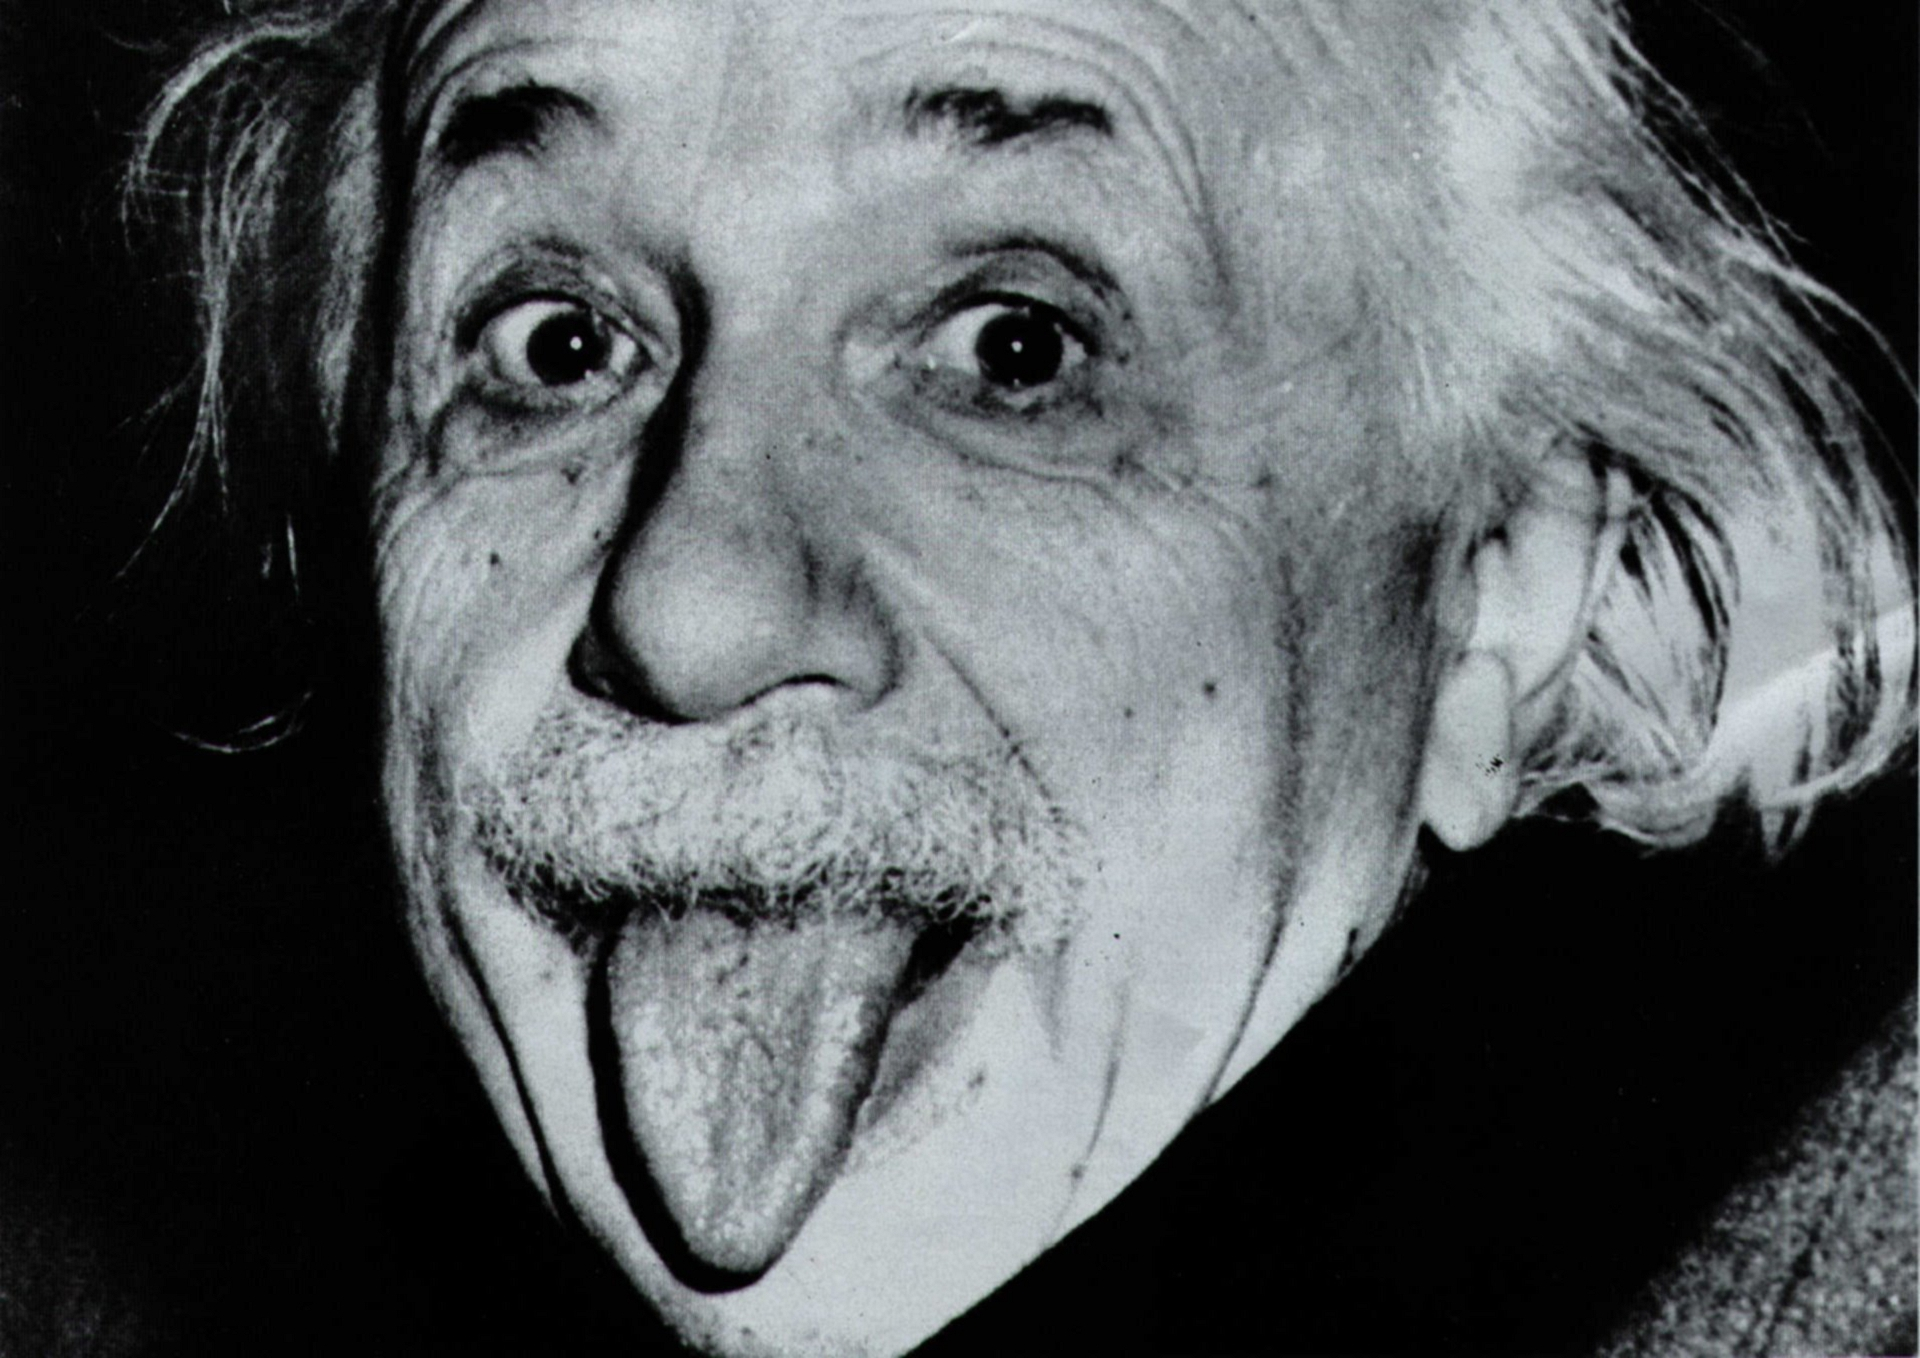
\includegraphics[width=0.9\linewidth]{Figures/Chapter2/einstein.jpeg}
    \caption{Albert Einstein}
    \label{fig:einstein}
\end{figure}

\subsection{Table}
Use table generator \url{https://www.tablesgenerator.com/} and paste it to display tables.

\subsection{Citation}
You can refer to previous works with cite command\cite{maiman1960stimulated}. The argument inside cite command can be multiple delimited by comma. The cited reference materials will be displayed in the Bibliography automatically ordered by appearance.
	%\input{Parts/Chapter3}
	%\input{Parts/Chapter4}
	%\input{Parts/Chapter5}



    \printbibliography[title=Bibliography]

\end{document}